\documentclass[logo,reportComp]{thesis}
\usepackage[cpp,pseudo]{mypackage}

\title{操作系统原理实验报告}
\subtitle{实验二:加载用户程序的监控程序}
\school{数据科学与计算机学院}
\author{陈鸿峥}
\classname{17大数据与人工智能}
\stunum{17341015}
\headercontext{操作系统原理实验报告}
\authorremark{本实验报告用\LaTeX撰写,创建时间:\builddate\today}


\begin{document}

\maketitle

\section{实验目的}
% 执行.com程序的批处理系统
% 1. 掌握COM格式的一种可执行程序的结构和运行要求。
% 2. 实现操作系统执行用户程序这一任务,理解操作系统产生的原始动机之一:自动执行用户程序,提高计算机的利用效率
% 3. 了解IBM_PC计算机硬件系统的内存布局和磁盘结构,设计一种简单的内存逻辑组织方法和磁盘组织方法,实现用户程序的存储。
% 4. 建立具有简单控制命令的批处理原型操作系统。
\begin{itemize}
	\item 实现一个最原始的操作系统,即一监控程序,用于调用执行用户程序
    \item 了解\verb'.com'格式文件的结构与作用
	\item 学会组织并存储监控程序和用户程序
\end{itemize}

\section{实验要求}
% 实验目的和实验要求由老师提供实验项目文档中获取
\begin{itemize}
	\item 设计四个(或更多)有输出的用户可执行程序\\
	设计四个有输出的用户可执行程序,分别在屏幕1/4区域动态输出字符,如展示实验一的内容:
	用字符‘A’从屏幕左边某行位置45度角下斜射出,保持一个可观察的适当速度直线运动,碰到屏幕相应1/4区域的边后产生反射,改变方向运动,如此类推,不断运动;在此基础上,增加个性扩展,还要在屏幕某个区域特别的方式显示学号姓名等个人信息
	\item 修改参考原型代码,允许键盘输入,用于指定运行这四个有输出的用户可执行程序之一,要确保系统执行代码不超过512字节,以便放在引导扇区
\end{itemize}
注意:自行组织映像盘的空间存放四个用户可执行程序

\section{实验环境}
% 包括:硬件或虚拟机配置方法、软件工具与作用、方案的思想、相关原理、程序流程、算法和数据结构、程序关键模块,结合代码与程序中的位置位置进行解释。不得抄袭,否则按作弊处理。
% 实验方案包括相关基础原理、实验工具和环境、程序流程和算法思想、数据结构与程序模块功能说明,代码文档组成说明等
具体环境选择原因已在实验一报告中说明。
\begin{itemize}
	\item Windows 10系统 + Ubuntu 18.04(LTS)子系统
	\item gcc 7.3.0 + nasm 2.13.02 + gdb
	\item Oracle VM VirtualBox 5.2.8
	\item Sublime Text 3
\end{itemize}

虚拟机配置:内存4M,无硬盘,1.44M虚拟软盘引导。

\section{实验方案}
% 包括:主要工具安装使用过程及截图结果、程序过程中的操作步骤、测试数据、输入及输出说明、遇到的问题及解决情况、关键功能或操作的截图结果。不得抄袭,否则按作弊处理。
\subsection{监控程序}
\subsubsection{主引导程序}
与实验一相同,虚拟软盘的第一个扇区用于存储主引导程序(即监控程序),需要保证最后两个字节为\verb'55aa'。
当验证主引导程序有效后,将会跳转到\verb'0x0000:0x7c00h'开始执行。

\subsubsection{调用并执行用户程序}
调用用户程序是实验二的核心内容,采用BIOS进行中断。

BIOS中已经含有磁盘读写的调用,即中断号13H和功能号02H的中断。
首先设置功能码(ah=2),要调用的程序占用的扇区数量(al=1),读取方式(软盘,dl=0),磁头号(dh=0),柱面号(ch=0),扇区开始编号(cl=[sectorNum]\footnote{这里采用了一个变量sectorNum,因有多个程序。}),读入数据在内存中的存储地址(\verb'[es:bx]')。

设置好上面的变量之后,调用13H中断(\verb'int 13H'),则此时磁盘中一个扇区的程序已经被读入内存。
接着跳转到用户程序执行。

注意这里需要先设置用户程序的偏移量(\verb'OffSetOfUserPrg=0A100h'),将\verb'OffSetOfUserPrg'赋值给\verb'bx',否则数据段位置不正确,用户程序将无法正常执行。

\subsubsection{字符串显示}
这里调用了自己写的\verb'showstring'函数,里面同样调用了BIOS中断(10号),可以直接将整个字符串在显存中显示出来。
详情见程序。

\subsection{用户程序}
一共4个用户程序,分别为\verb'prg1.com'到\verb'prg4.com'。

\subsubsection{程序功能}
这里复用了实验一的程序,详情请见实验一的实验报告。
但是每个程序会有一定的区别,具体如下:
\begin{itemize}
	\item 程序一:最简单的单字符反弹无变色显示
	\item 程序二:两个字符的V形复杂变色显示
	\item 程序三:连续两个字符(`OS')不闪烁的变色显示
	\item 程序四:两个字符的平行四边形复杂变色显示
\end{itemize}

同时,每个程序只占用1/4的显存区域,这可以从每个程序最前面的常量(\verb'minX'、\verb'minY'、\verb'maxX'、\verb'maxY')设置更改。

\subsubsection{存储组织}
主引导程序存储在虚拟软盘的第一个扇区,第一个用户程序存储在第二个扇区,第二个用户程序存储在第三个扇区,以此类推。

注意在每个用户程序开头都应该加上\verb'org 0A100h',与前面的\verb'OffSetOfUserPrg'相同,表明用户程序读入内存应从内存物理地址\verb'0A100h'开始。

\subsubsection{返回监控程序}
DOS环境下中断向量表存放在物理地址\verb'0x0000'到\verb'0x03ff',大小为1KB(1024B)。
每个中断在中断向量表中占4B,高位为中断处理程序的段地址(segment),低位为中断处理程序的偏移量(offset)。
且每个中断对应着一个中断标号(\verb'int'),如除以0中断为\verb'0x0000-0x0003',用\verb'int 0'调用。
因此计算标号为$i$的中断入口地址可以通过$i\times 4$得到。

通过wiki得知,中断标号\verb'0x00'到\verb'0x13'已经具有功能,\verb'0x14'到\verb'0x1f'为保留标号,\verb'0x20'到\verb'0xff'提供给用户自定义中断。
因此,我定义了\verb'0x20h'号中断(用上面计算地址的方法将返回函数地址放入中断向量表),用于从用户程序返回监控程序。

做法是用\verb'int 16'中断监测用户是否有键入Ctrl+C(扫描码\verb'2e03h'),如果有则返回监控程序。

并且,在每个用户程序的\verb'show'循环中要加入软件中断\verb'int 20h',用于监测是否有键盘返回,如果有则清空显存并返回监控程序,否则则继续执行该用户程序。

\subsection{镜像文件写入}
由于一共有5个程序需要编译并写入,如果每次都要重新输入命令则非常麻烦。

因此在这里本人自己写了一个Linux环境下的批处理程序\verb'work.sh',用于虚拟软盘的创建、汇编程序的编译与写入,如下所示。
\begin{lstlisting}[language=bash]
#!/bin/bash

rm mydisk.img
/sbin/mkfs.msdos -C mydisk.img 1440
nasm os.asm -o os.com
dd if=os.com of=mydisk.img conv=notrunc
nasm prg1.asm -o prg1.com
dd if=prg1.com of=mydisk.img seek=1 conv=notrunc
nasm prg2.asm -o prg2.com
dd if=prg2.com of=mydisk.img seek=2 conv=notrunc
nasm prg3.asm -o prg3.com
dd if=prg3.com of=mydisk.img seek=3 conv=notrunc
nasm prg4.asm -o prg4.com
dd if=prg4.com of=mydisk.img seek=4 conv=notrunc
\end{lstlisting}

\section{实验结果}
调用\verb'work.sh'生成虚拟软盘\verb'mydisk.img',批处理程序执行截图如图\ref{fig:sh}所示。
\begin{figure}[H]
\centering
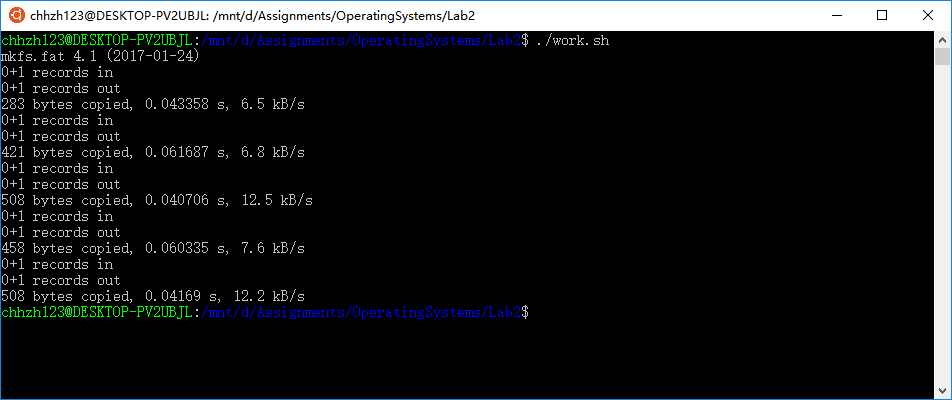
\includegraphics[width=\linewidth]{fig/sh.PNG}
\caption{Linux批处理程序}
\label{fig:sh}
\end{figure}

将生成的\verb'mydisk.img'加载入虚拟机运行。

首先进入的是监控程序,如图\ref{fig:monitor}所示。
输入数字$1\thicksim 4$,可以选择不同的用户程序。
各用户程序的功能已在前面说明,结果如图\ref{fig:1}到图\ref{fig:4}所示。
\begin{figure}[H]
\centering
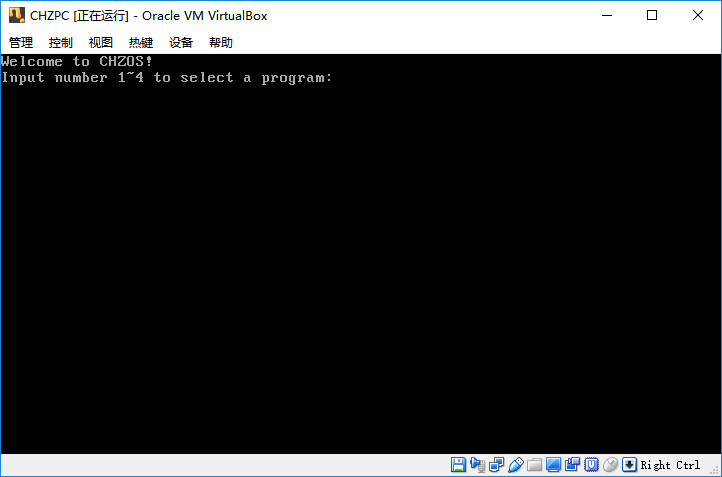
\includegraphics[width=\linewidth]{fig/monitor.PNG}
\caption{监控程序入口}
\label{fig:monitor}
\end{figure}
\begin{figure}[H]
\centering
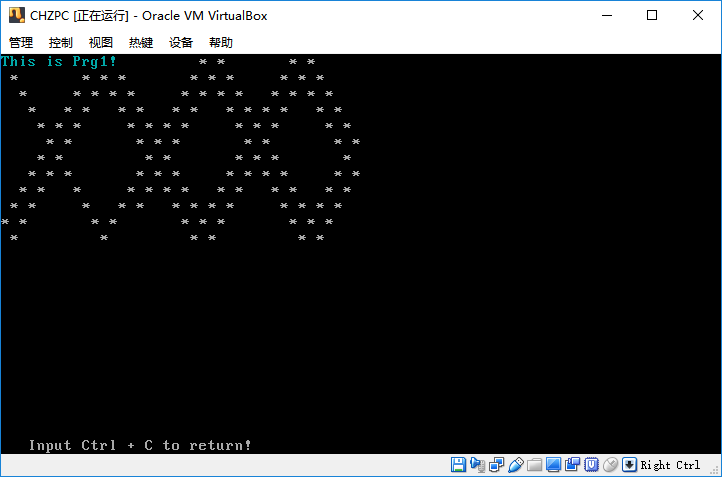
\includegraphics[width=\linewidth]{fig/prg1.PNG}
\caption{用户程序1}
\label{fig:1}
\end{figure}
\begin{figure}[H]
\centering
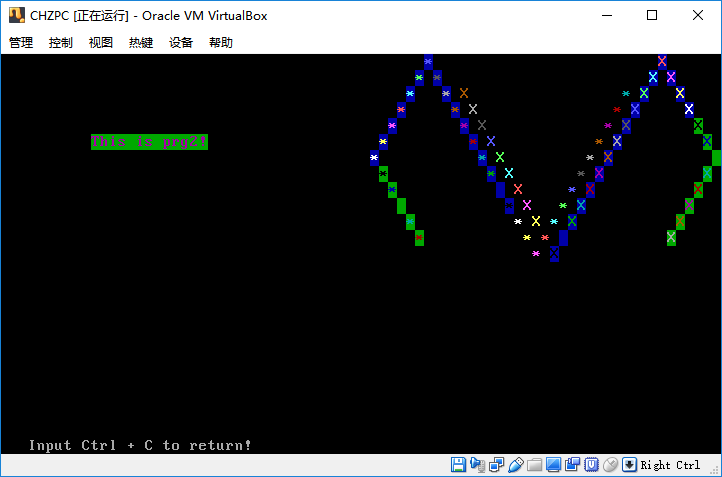
\includegraphics[width=\linewidth]{fig/prg2.PNG}
\caption{用户程序2}
\label{fig:2}
\end{figure}
\begin{figure}[H]
\centering
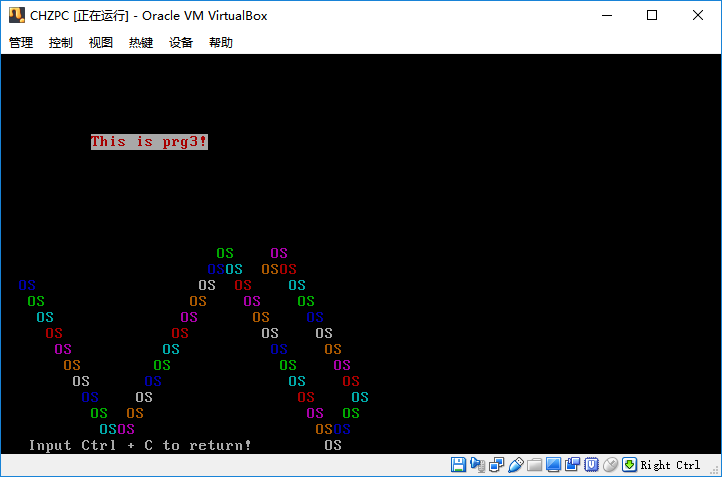
\includegraphics[width=\linewidth]{fig/prg3.PNG}
\caption{用户程序3}
\label{fig:3}
\end{figure}
\begin{figure}[H]
\centering
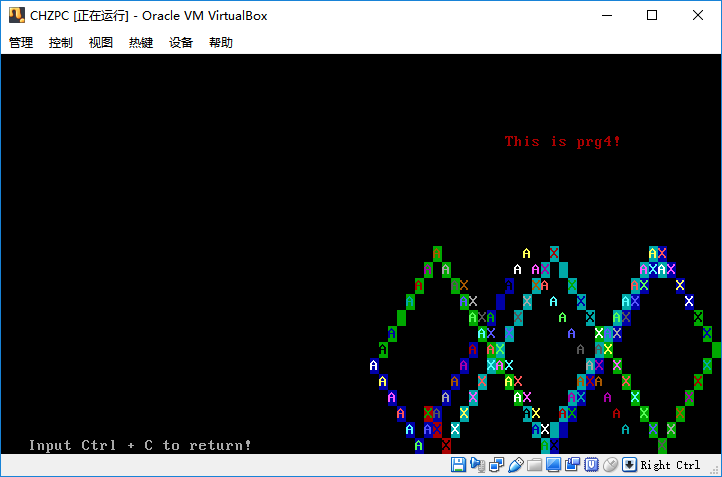
\includegraphics[width=\linewidth]{fig/prg4.PNG}
\caption{用户程序4}
\label{fig:4}
\end{figure}

\section{实验总结}
% 每人必需写一段,文字不少于500字,可以写心得体会、问题讨论与思考、新的设想、感言总结或提出建议等等。不得抄袭,否则按作弊处理。

第二次实验有了第一次实验的基础,会相对好做很多。

这次牢记上次实验的bug,注意到一定要在主引导程序中添加\verb'org 7c00h'指令,以告诉汇编器加载入指令和数据到内存的位置。
由于虚拟机会将虚拟软盘第0面第0道第1扇区的512B的程序(主引导程序)加载到\verb'7c00h'处,如果不添加\verb'org'指令,则主引导程序指令的段内偏移错误,程序将无法正常运行。
虽然记得在监控程序中添加\verb'org',但本次实验一开始还是在用户程序中忘记添加\verb'org 0A100h',导致程序调用无法正常进行,说到底还是对\verb'org'的理解不够透彻。
既然在监控程序中告诉BIOS将用户程序需加载到内存\verb'0A100h'的位置,即段内偏移起始地址变化了,那么在用户程序中也需要声明这一点,因此才要在每个用户程序内添加\verb'org 0A100h'。

这次一共编写了5个汇编程序,更加了解到x86 CPU寄存器的分配及使用应该怎么办,特别是写中断的时候,常常会怀疑寄存器够不够用,这一点就要合理利用寄存器,把长的寄存器拆分成几个小的寄存器,分开用。
如把32位的\verb'eax',拆分为16位的\verb'ax';16位的\verb'ax'又可拆分为高8位的\verb'ah'和低8位的\verb'al'。
从这一点也可以看出,当今的编译器的功能多么强大,竟然可以将我们那么复杂的高级语言程序中的变量,合理地映射到各个寄存器上进行计算。

然后则是,写Linux批处理文件\verb'.sh'时出现的问题。
由于我用的是子系统,编写代码程序时依然在Windows环境下进行,因此没有注意到Windows环境和Linux环境下文本文档的区别。
Windows环境默认换行采用两个字符,即\verb'\r\n',而Linux环境则是单个字符\verb'\n'。
对于批处理程序来说,对字符相当敏感,因而在执行过程中会报错,无法识别
好在Sublime Text 3本来就可以设置编辑的选项,点击Preferences-Settings,在弹出的\verb'Preferences.sublime-settings'文件中,添加\verb'"default_line_ending": "unix"'即可实现在Windows环境下编写代码但采用的是Linux环境的换行符。

为了增强程序的鲁棒性,在本次实验中我也添加了一些异常处理机制,如在读取用户输入过程中,判断用户输入是否有效,如果无效则另用户重新输入,有效才开始执行下一步操作。

总的来说,本次实验自己实现了一个最为简单的操作系统,实现调取执行用户程序的功能,了解\verb'.com'格式文件的组织和作用,更加深刻明白了\verb'org'的含义,以及x86汇编的编写。
感受颇深,也非常兴奋,希望通过这样子不断地训练,最终真的可以写出一个完整的操作系统出来。

\section{参考资料}
\begin{enumerate}
	\item 李忠,王晓波,余洁,《x86汇编语言-从实模式到保护模式》,电子工业出版社,2013
	\item 中断向量表(IVT),\url{https://wiki.osdev.org/Interrupt_Vector_Table}
	\item DOS的古董美,\url{http://www.voidcn.com/article/p-tabpatgs-ps.html}
	\item INT 16 - Keyboard Scan Codes, \url{http://stanislavs.org/helppc/scan_codes.html}
	\item \verb'iret', \url{https://www.felixcloutier.com/x86/iret:iretd}
	\item (x86 Assembly) Changing Interrupt Vector Table, \url{http://devdocs.inightmare.org/tutorials/x86-assembly-changing-interrupt-vector-table.html}
    \item org指令的作用,\url{https://blog.csdn.net/mirage1993/article/details/29908929}
    % \item Sublime settings, \url{https://blog.csdn.net/fanlying/article/details/79743178}
\end{enumerate}

\appendix
\appendixconfig
\section{程序清单}
\label{sec:code}
这里只附上主引导程序的代码,其他用户程序请见附件。
\begin{lstlisting}[language={[x86masm]Assembler}]
; Constants
OffSetOfUserPrg equ 0A100h

;;;;; Initialization ;;;;;
    org  7c00h

;;;;; Initializeion ;;;;;
%macro showstring 4
    ; msg, msglen, row, col
    mov ax, cs               ; as = cs
    mov ds, ax               ; data segment
    mov bp, %1               ; bp = string index
    mov ax, ds               ; (BIOS) es:bp = string address
    mov es, ax               ; es = ax
    mov cx, %2               ; (BIOS) set string length
    mov ax, 1301h            ; (BIOS) ah = 13h (BIOS: function code) al = 01h (only char)
    mov bx, 0007h            ; (BIOS) page/bh = 00h property/bl = 07h
    mov dh, %3               ; (BIOS) row
    mov dl, %4               ; (BIOS) col
    int 10h                  ; (BIOS) 10h: show one string
%endmacro

%macro writeIVT 2            ; write interrupt vector table (IVT)
    ; num, function address
    mov ax, 0000h            ; physical address
    mov es, ax
    mov ax, %1
    mov bx, 4
    mul bx                   ; calculate the IVT address (ax*4)
    mov si, ax
    mov ax, %2
    mov [es:si], ax          ; write segment
    add si, 2
    mov ax, cs
    mov [es:si], ax          ; write offset
%endmacro

writeIVT 20h, INT20H

begin:
    showstring msg, msglen, 0, 0
    showstring msg2, msglen2, 1, 0

input:
    mov ah, 0                ; (BIOS) function code
    int 16h                  ; (BIOS) read keyboard
    sub al, '0'              ; (BIOS) return al = ASCII
    cmp al, 1
    jl input                 ; not from 1~4
    cmp al, 4
    jg input                 ; not from 1~4
    inc al                   ; start from 2
    mov [sectorNum], al      ; put it into memory

;;;;; Load Program ;;;;;
load:                        ; load [es:bx]
    call clear               ; clear the screen
    mov ax, cs               ; segment address (store data)
    mov es, ax               ; set segment
    mov bx, OffSetOfUserPrg  ; user program address
    mov ah, 2                ; (BIOS) function code
    mov al, 1                ; (BIOS) # of sector that program used
    mov dl, 0                ; (BIOS) driver: floppy disk (0)
    mov dh, 0                ; (BIOS) magnetic head
    mov ch, 0                ; (BIOS) cylinder
    mov cl, [sectorNum]      ; (BIOS) start sector
    int 13H                  ; (BIOS) 13h: read disk
    jmp OffSetOfUserPrg      ; a.com has been loaded into memory

clear:
    mov ax, 0B800h           ; video memory
    mov es, ax
    mov si, 0
    mov cx, 80*25
    mov dx, 0
    clearloop:
        mov [es:si], dx
        add si, 2
    loop clearloop
    ret

INT20H:
    showstring msg3, msglen3, 24, 3
    mov ah, 01h
    int 16h
    jz noclick
    mov ah, 00h               ; click the button
    int 16h
    cmp ax, 2e03h             ; click Ctrl + C
    jne noclick
    call clear                ; clear the screen
    jmp begin                 ; return to monitor program
    noclick:
    iret                      ; interrupt return

end:
    jmp $

;;;;; Data Segment ;;;;;
datadef:
    msg db 'Welcome to CHZOS!'
    msglen equ ($-msg)

    msg2 db 'Input number 1~4 to select a program: '
    msglen2 equ ($-msg2)

    msg3 db 'Input Ctrl + C to return!'
    msglen3 equ ($-msg3)

    sectorNum db '1'
\end{lstlisting}

\section{附件文件说明}
\begin{center}
\begin{tabular}{|c|l|l|}\hline
序号 & 文件 & 描述 \\\hline
1 & \verb'os.asm' & 主引导程序 \\\hline
2 & \verb'os.com' & 主引导程序编译出来的\verb'.com'执行文件\\\hline
3-6 & \verb'prgX.asm' & 四个用户程序\\\hline
7-10 & \verb'prgX.com' & 四个用户程序编译出来的\verb'.com'执行文件\\\hline
11 & \verb'work.sh' & Linux环境批处理代码\\\hline
12 & \verb'mydisk.img' & 我的OS虚拟软盘(里面已包含程序)\\\hline
\end{tabular}
\end{center}

\end{document}

% 实验提交内容
% 实验报告:电子版(Word2003的DOC格式或PDF格式)
% 原程序文件及可执行代码程序文件
% 测试输入数据文件和输出数据文件
% 虚拟机软盘映像文件

% 基础实验项目5个和扩展实验7个
% 实验项目,迟交影响成绩评价!
% 工具与环境可由选择,开发新型工具或优化一套开发环境都可加分!
% 一系列基础实验项目必须连续完成,当前项目只能在前一个项目的基础上进行,体现出前后的进化关系,否则要被约谈,证明没有抄袭行为!
% 一个项目可提交多个改进的版本,实现新功能和个性化特征都有利于提高相应项目的成绩。
% 实验项目提交内容用winrar工具整体压缩打包,统一格式命名为:
%    <学号>+<姓名>+<实验项目号>+<版本号>.rar

% 免考
% 条件:实验1~6全部评价AAAAB+B+或相当
% 最终成绩可能范围:75分以上